\chapter{Bactériologie~: croissance, physiologie et génétique}\label{ch:b3:bacteriology}

Une seule cellule d'\emph{Escherichia coli} dans un bouillon tiède se
divise toutes les vingt minutes. Sans frein, sa descendance pèserait
plus que la Terre en deux jours~; en réalité elle s'arrête en quelques
heures, quand le sucre vient à manquer, et demeure des semaines dans un
état qui survit à la famine. Une bactérie voisine, dans une plaie et en
quelques heures, devient cent millions de cellules et une fièvre~; il y
a cent ans elle tuait un tiers des patients qu'elle infectait, et depuis
1941 le poison d'une moisissure contre elle a sauvé plus de vies que
n'importe quel autre médicament --- tandis que les bactéries, pendant
ces quatre-vingts mêmes années, ont trouvé le moyen de contourner tous
les \omterm{def:b3:bacteriology:antibiotics}{antibiotiques} fabriqués. Les bactéries sont les organismes chez qui
l'on a montré pour la première fois que les gènes sont de l'ADN, chez
qui la régulation des gènes a été comprise pour la première fois, et
auxquels on a pris les outils du \cref{ch:b3:genetic-engineering}. Ce
chapitre les traite en tant qu'organismes~: leur enveloppe,
l'arithmétique de leur croissance dans un flacon et en culture
continue, la façon dont une population perçoit sa propre densité, le
trafic des gènes entre cellules, et la chimie et l'évolution des
\omterm{def:b3:bacteriology:antibiotics}{antibiotiques} et des résistances.

\section{La cellule bactérienne}

\begin{definition}[L'enveloppe]\label{def:b3:bacteriology:envelope}
\index{peptidoglycane}\index{Gram positif}\index{Gram négatif}\index{membrane externe}\index{lipopolysaccharide}\index{endospore}
Toute bactérie, à quelques exceptions près, est enfermée dans une paroi
de \emph{peptidoglycane}~: des chaînes alternant N-acétylglucosamine et
acide N-acétylmuramique, réticulées par de courts peptides en une seule
molécule qui entoure la cellule et résiste à la pression de turgescence
--- plusieurs atmosphères --- du cytoplasme. Les bactéries \emph{à Gram
positif} ont une paroi épaisse de \qtyrange{20}{80}{nm}, à nombreuses
couches, traversée d'acides téichoïques~; les bactéries \emph{à Gram
négatif} ont une paroi mince d'une ou deux couches et, à l'extérieur,
une seconde bicouche lipidique, la \emph{membrane externe}, dont le
feuillet externe est du \emph{lipopolysaccharide} (LPS, endotoxine ---
la molécule que reconnaît le système immunitaire inné du
\cref{ch:b3:innate-immunity} et qui cause le choc septique), et qui
enferme un périplasme. Des porines de la membrane externe laissent
entrer les petites molécules et excluent bien des \omterm{def:b3:bacteriology:antibiotics}{antibiotiques}. À
l'extérieur peuvent se trouver une capsule polysaccharidique contre les
phagocytes, des flagelles pour nager
(\cref{ch:b3:cytoskeleton-motility}) et des pili pour l'attachement et
la \omterm{def:b3:bacteriology:hgt}{conjugaison}. À l'intérieur, le chromosome --- une molécule
circulaire de \qtyrange{1}{10}{Mb} chez la plupart des espèces --- est
replié en un nucléoïde dépourvu de membrane, à côté de \omterm{def:b3:genetic-engineering:tools}{plasmides}.
Certains genres (\emph{Bacillus}, \emph{Clostridium}) savent enfermer
une copie du chromosome dans une enveloppe épaisse, en
\emph{endospore}, déshydratée et métaboliquement inerte, qui survit à
l'ébullition, aux rayonnements et à des siècles de sécheresse et germe
au retour des nutriments.
\end{definition}

\begin{method}[La coloration de Gram]\label{met:b3:bacteriology:gram}
\index{coloration de Gram}
Le plus vieux test du laboratoire de bactériologie (Gram, 1884) décide
encore du premier choix d'\omterm{def:b3:bacteriology:antibiotics}{antibiotique}. (1) Étaler l'échantillon et le
fixer à la chaleur~; (2) colorer au violet de gentiane, puis à l'iode,
qui forme avec le colorant un gros complexe insoluble à l'intérieur des
cellules~; (3) laver à l'alcool~: l'épais \omterm{def:b3:bacteriology:envelope}{peptidoglycane} des \omterm{def:b3:bacteriology:envelope}{Gram
positifs}, déshydraté par l'alcool, retient le complexe et les cellules
restent violettes, alors que la paroi mince des \omterm{def:b3:bacteriology:envelope}{Gram négatifs} le laisse
sortir~; (4) contre-colorer à la safranine, qui rose les \omterm{def:b3:bacteriology:envelope}{Gram négatifs}
devenus incolores. La forme et la disposition --- coques en amas
(staphylocoques) ou en chaînes (streptocoques), bâtonnets, spirales ---
resserrent encore l'identification, et un coque violet en amas provenant
d'un abcès est un staphylocoque avant toute culture.
\end{method}

\begin{omfigure}
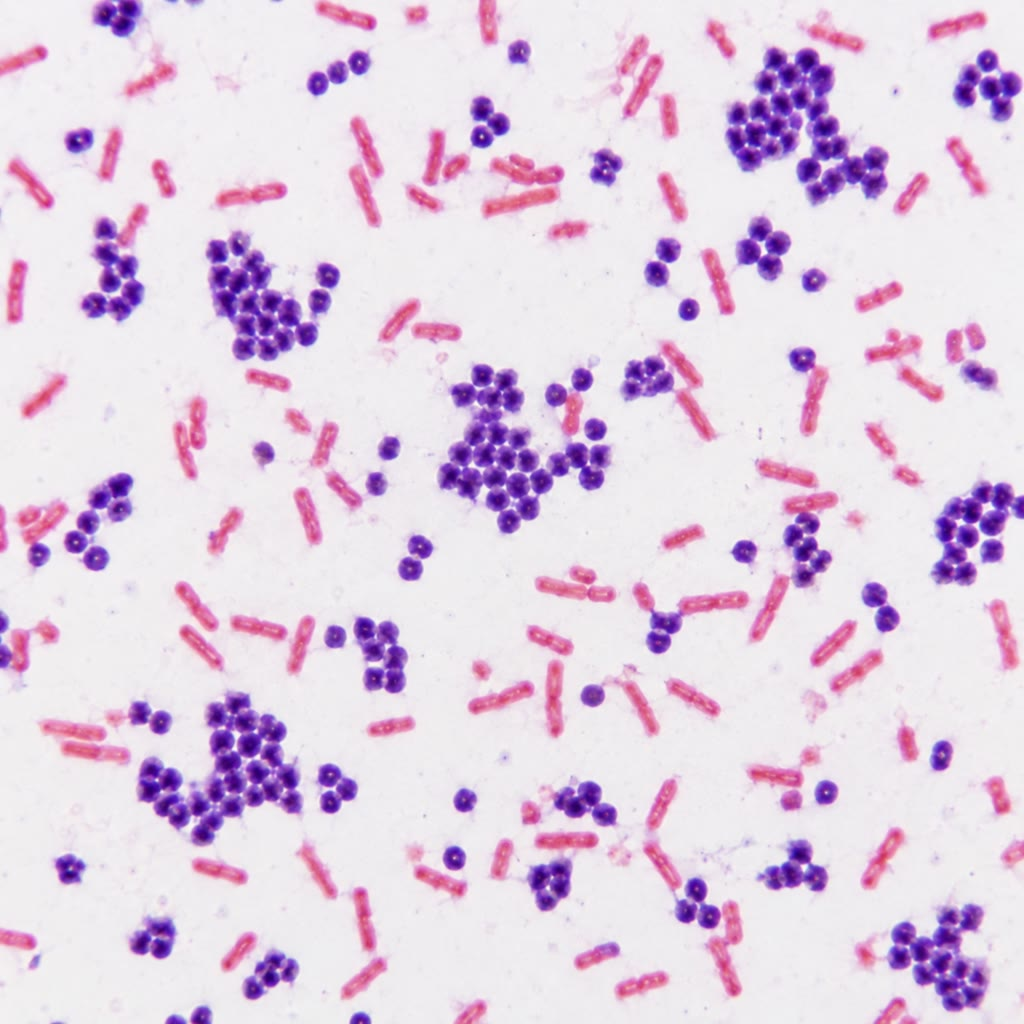
\includegraphics[width=0.36\linewidth]{images/book5/ai/b5-12-gram-stain.jpg}\hspace{0.04\linewidth}
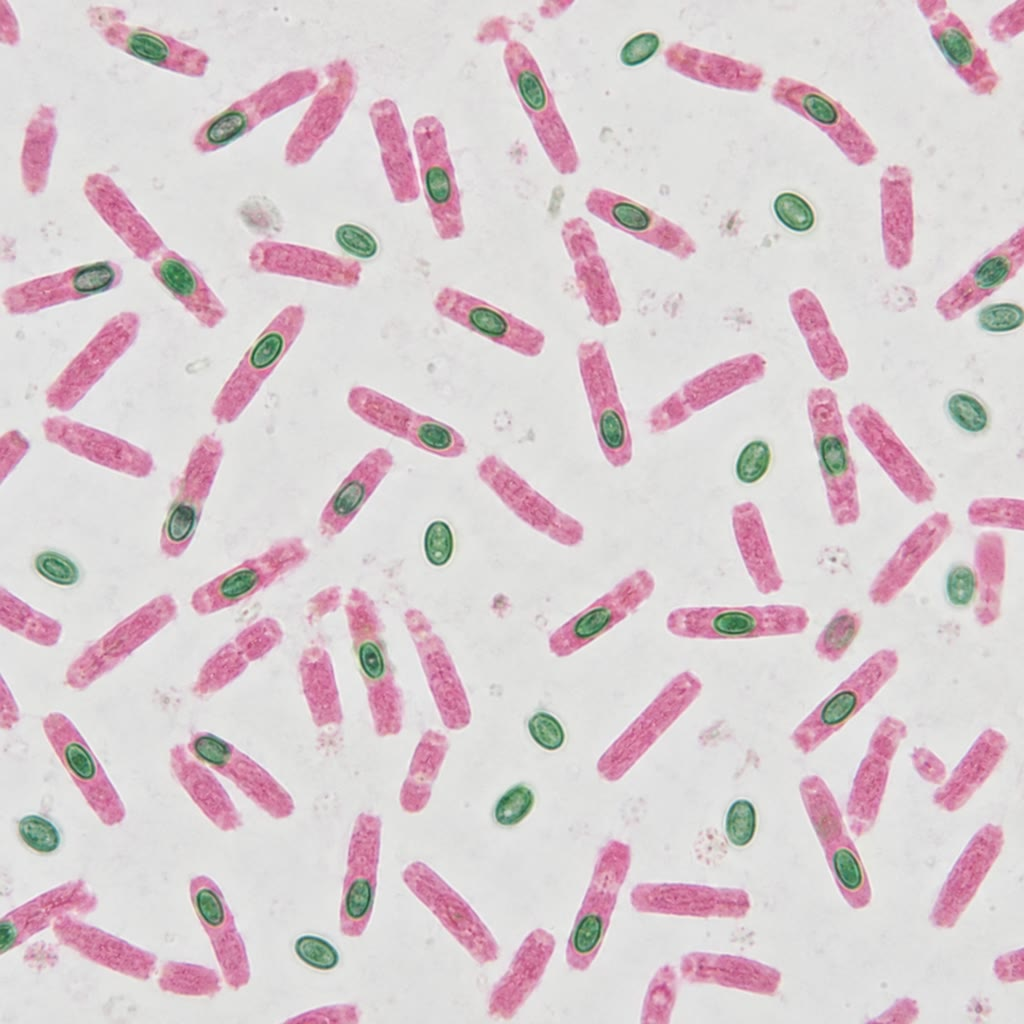
\includegraphics[width=0.36\linewidth]{images/book5/ai/b5-12-endospores.jpg}

{\small À gauche~: une \omterm{met:b3:bacteriology:gram}{coloration de Gram} --- coques à \omterm{def:b3:bacteriology:envelope}{Gram positif}
violets en amas, bâtonnets à \omterm{def:b3:bacteriology:envelope}{Gram négatif} roses. À droite~: des
cellules de \emph{Bacillus} colorées pour les \omterm{def:b3:bacteriology:envelope}{endospores}, ovales vert
vif à l'intérieur de cellules roses et spores libres à côté d'elles.}
\end{omfigure}

\begin{omfigure}
\begin{tikzpicture}[every node/.style={font=\scriptsize}, >=stealth]
  % Gram-positive
  \begin{scope}
    \fill[omDef!15] (0,0) rectangle (4.5,0.4); \draw[thick, omDef] (0,0) -- (4.5,0); \draw[thick, omDef] (0,0.4) -- (4.5,0.4);
    \fill[omProp!40] (0,0.5) rectangle (4.5,2.0); \foreach \y in {0.7,0.95,1.2,1.45,1.7} \draw[omProp!80!black, thin] (0,\y) -- (4.5,\y);
    \foreach \x in {0.6,1.6,2.6,3.6} \draw[omMeth!70!black, thick] (\x,0.5) -- (\x,2.3);
    \node[below] at (2.25,-0.1) {membrane cytoplasmique};
    \node[right, align=left] at (4.6,1.25) {peptidoglycane épais\\(\qtyrange{20}{80}{nm})}; \node[right, omMeth!70!black] at (4.6,2.2) {acides téichoïques};
    \node[above, font=\small\bfseries] at (2.25,2.5) {Gram positif};
  \end{scope}
  % Gram-negative
  \begin{scope}[xshift=8.6cm]
    \fill[omDef!15] (0,0) rectangle (4.5,0.4); \draw[thick, omDef] (0,0) -- (4.5,0); \draw[thick, omDef] (0,0.4) -- (4.5,0.4);
    \fill[omProp!40] (0,0.75) rectangle (4.5,1.05); \draw[omProp!80!black, thin] (0,0.9) -- (4.5,0.9);
    \fill[omDef!15] (0,1.5) rectangle (4.5,1.9); \draw[thick, omDef] (0,1.5) -- (4.5,1.5); \draw[thick, omDef] (0,1.9) -- (4.5,1.9);
    \foreach \x in {0.4,0.9,1.4,1.9,2.4,2.9,3.4,3.9} \draw[omThm, thick] (\x,1.9) -- (\x,2.35);
    \draw[thick, fill=white] (2.0,1.45) rectangle (2.5,1.95); \node[below, font=\tiny] at (2.25,1.45) {porine};
    \node[below] at (2.25,-0.1) {membrane cytoplasmique};
    \node[right] at (4.6,0.9) {peptidoglycane mince}; \node[right] at (4.6,1.7) {membrane externe}; \node[right, omThm] at (4.6,2.25) {LPS (endotoxine)};
    \node[right, font=\tiny] at (4.6,1.27) {périplasme};
    \node[above, font=\small\bfseries] at (2.25,2.5) {Gram négatif};
  \end{scope}
\end{tikzpicture}

{\small Les deux enveloppes. Les \omterm{def:b3:bacteriology:envelope}{Gram positifs} enveloppent la membrane
de nombreuses couches de \omterm{def:b3:bacteriology:envelope}{peptidoglycane}~; les \omterm{def:b3:bacteriology:envelope}{Gram négatifs} ont une
couche mince et une \omterm{def:b3:bacteriology:envelope}{membrane externe} de \omterm{def:b3:bacteriology:envelope}{lipopolysaccharide} percée de
porines, qui tient bien des \omterm{def:b3:bacteriology:antibiotics}{antibiotiques} à l'écart et fournit
l'endotoxine qui cause le choc septique.}
\end{omfigure}

\section{La croissance}

\begin{theorem}[Croissance exponentielle, loi de Monod et chémostat]\label{thm:b3:bacteriology:monod}
\index{croissance exponentielle!bactéries}\index{équation de Monod}\index{chémostat}\index{taux de dilution}
Une population de $N$ cellules qui se divisent avec le temps de
génération $T$ croît comme $N(t) = N_{0}\,2^{t/T} = N_{0}e^{\mu t}$,
avec le taux de croissance spécifique $\mu =
\ln 2/T$. Ce taux dépend du nutriment limitant $S$ par la \emph{loi de
Monod}
\[
\mu(S) = \mu_{\max}\,\frac{S}{K_{S} + S},
\]
qui sature à $\mu_{\max}$ et vaut la moitié du maximum en $S = K_{S}$.
Dans un \emph{chémostat} --- une cuve de volume $V$ où entre un milieu
neuf de concentration en nutriment $S_{0}$ à la vitesse $F$, et d'où la
culture sort à la même vitesse, avec le \omterm{thm:b3:bacteriology:monod}{taux de dilution} $D = F/V$ ---
l'état stationnaire vérifie
\[
\mu(S^{*}) = D,\qquad S^{*} = \frac{K_{S}D}{\mu_{\max} - D},\qquad
X^{*} = Y\,(S_{0} - S^{*}),
\]
où $X$ est la densité cellulaire et $Y$ le rendement (cellules
produites par unité de nutriment). L'expérimentateur fixe le taux de
croissance en réglant une pompe~; la culture répond en ajustant le
nutriment qu'elle laisse derrière elle. Si $D$ dépasse $\mu(S_{0})$ les
cellules ne peuvent plus suivre et sont lessivées.
\end{theorem}
\begin{proof}
Cellules~: $\mathrm{d}X/\mathrm{d}t = \mu(S)X - DX$, croissance moins
sortie~; à l'état stationnaire avec $X^{*} > 0$, $\mu(S^{*}) = D$, et
inverser la loi de Monod donne $S^{*}$. Nutriment~:
$\mathrm{d}S/\mathrm{d}t = D(S_{0} -
S) - \mu(S)X/Y$, entrée moins sortie moins consommation~; à l'état
stationnaire, avec $\mu = D$, $D(S_{0} - S^{*}) = DX^{*}/Y$, d'où
$X^{*}$. L'état stationnaire n'existe que si $S^{*} < S_{0}$,
c'est-à-dire $D <
\mu(S_{0})$~; au-delà, le seul état stationnaire est $X = 0$, le
lessivage. Stabilité~: si $X$ monte au-dessus de $X^{*}$ il consomme
davantage, $S$ tombe sous $S^{*}$, $\mu$ tombe sous $D$ et $X$ décline
--- une rétroaction négative par le nutriment.
\end{proof}

\begin{example}[Une culture en chiffres]\label{ex:b3:bacteriology:numbers}
\emph{E.~coli} en milieu riche à \qty{37}{\celsius}~: $T = \qty{20}{min}$,
$\mu = \qty{2.1}{h^{-1}}$. À partir d'une cellule, $2^{36}$ après douze
heures --- $7\times 10^{10}$ cellules, soit environ \qty{70}{mg}, ce
qui est le point où un flacon de \qty{100}{mL} s'arrête faute de
dioxygène et de sucre~; la «~masse de la Terre en deux jours~» fait
$2^{144}\approx 10^{43}$ cellules, et l'arithmétique ne montre qu'une
chose~: la croissance exponentielle ne dure jamais. Dans un chémostat
sur glucose avec $\mu_{\max} = \qty{1.0}{h^{-1}}$, $K_{S} =
\qty{0.01}{g/L}$, $S_{0} = \qty{1}{g/L}$ et $Y = \qty{0.5}{g}$ de
cellules par gramme de glucose, un \omterm{thm:b3:bacteriology:monod}{taux de dilution} de
\qty{0.5}{h^{-1}} laisse $S^{*}
= 0.01\times 0.5/0.5 = \qty{0.01}{g/L}$ de glucose et maintient $X^{*} =
\qty{0.495}{g/L}$ de cellules, qui se divisent toutes les \qty{83}{min},
indéfiniment. Le chémostat est la façon d'étudier la physiologie à taux
de croissance fixé, et de faire tourner des milliers de générations
d'évolution dans une bouteille.
\end{example}

\begin{omfigure}
\begin{tikzpicture}
\begin{axis}[
  width=6.6cm, height=5.4cm,
  axis x line=bottom, axis y line=left,
  xmin=0, xmax=14, ymin=1e6, ymax=1e10, ymode=log,
  xlabel={heures}, ylabel={cellules par mL},
  xlabel style={font=\small, at={(axis description cs:0.5,-0.12)}, anchor=north}, ylabel style={font=\small},
  tick label style={font=\scriptsize}, xtick={0,4,8,12},
  clip=false,
]
\addplot[very thick, omDef, domain=0:1.5, samples=2] {1e6};
\addplot[very thick, omDef, domain=1.5:7.5, samples=40] {1e6*2^((x-1.5)/0.5)};
\addplot[very thick, omDef, domain=7.5:12, samples=2] {4.1e9};
\addplot[very thick, omDef, domain=12:14, samples=10] {4.1e9*exp(-0.15*(x-12))};
\node[font=\scriptsize, anchor=south] at (axis cs:0.8,1.2e6) {latence};
\node[font=\scriptsize, anchor=west] at (axis cs:2.5,3e8) {exponentielle~: $T = \qty{30}{min}$};
\node[font=\scriptsize, anchor=north] at (axis cs:10,3.5e9) {stationnaire};
\node[font=\scriptsize, anchor=north] at (axis cs:12.8,2.2e9) {mort};
\end{axis}
\begin{axis}[
  at={(7.8cm,0)}, anchor=south west,
  width=6.6cm, height=5.4cm,
  axis x line=bottom, axis y line=left,
  xmin=0, xmax=0.1, ymin=0, ymax=1.1,
  xlabel={glucose $S$ (g/L)}, ylabel={$\mu$ (h$^{-1}$)},
  xlabel style={font=\small, at={(axis description cs:0.5,-0.12)}, anchor=north}, ylabel style={font=\small},
  tick label style={font=\scriptsize}, xtick={0,0.01,0.05,0.1}, xticklabels={0,$K_S$,0.05,0.1}, ytick={0,0.5,1},
  clip=false,
]
\addplot[very thick, omThm, domain=0:0.1, samples=60] {x/(0.01+x)};
\addplot[dashed, gray, domain=0:0.1, samples=2] {1};
\addplot[dashed, gray] coordinates {(0.01,0) (0.01,0.5)}; \addplot[dashed, gray] coordinates {(0,0.5) (0.01,0.5)};
\node[font=\scriptsize, omThm, anchor=north west] at (axis cs:0.045,0.6) {Monod~: $\mu = \mu_{\max}S/(K_{S}+S)$};
\node[font=\scriptsize, gray, anchor=south east] at (axis cs:0.1,1.01) {$\mu_{\max}$};
\end{axis}
\end{tikzpicture}

{\small À gauche~: une culture en flacon --- une latence pendant que les
enzymes sont induites, une croissance exponentielle, une \omterm{def:b3:bacteriology:phases}{phase
stationnaire} quand le nutriment est épuisé, puis une mort lente. À
droite~: la loi de Monod, taux de croissance en fonction du nutriment
limitant, $K_{S}$ étant la concentration donnant la moitié du maximum.}
\end{omfigure}

\begin{definition}[Phases et états]\label{def:b3:bacteriology:phases}
\index{phase de latence}\index{phase stationnaire}\index{sporulation}\index{facteur sigma}
Dans un flacon neuf (une \emph{culture discontinue}) les cellules
marquent d'abord une pause --- la \emph{phase de latence}, le temps
d'induire les enzymes qu'exige le nouveau milieu --- puis croissent
exponentiellement, puis s'arrêtent quand un nutriment est épuisé ou
qu'un déchet s'accumule~: c'est la \emph{phase stationnaire}, où les
cellules rapetissent, épaississent leur enveloppe, condensent leur
nucléoïde autour de protéines protectrices, allument des gènes de
stress par le facteur sigma de rechange RpoS, et peuvent survivre des
mois~; suit une phase de mort où la plupart des cellules se lysent et
où quelques-unes vivent sur les restes. Certaines espèces répondent à
la famine par un programme de développement~: \emph{Bacillus subtilis}
se divise de façon asymétrique et la grande cellule englobe la petite
et bâtit la spore autour d'elle, une séquence de huit heures commandée
par une cascade de \emph{facteurs sigma} --- les sous-unités qui
dirigent l'ARN polymérase vers un jeu de promoteurs --- alternant entre
les deux compartiments, premier exemple bactérien de différenciation et
de signalisation de cellule à cellule au travers d'une paroi.
\end{definition}

\section{Se percevoir les unes les autres}

\begin{definition}[Détection du quorum]\label{def:b3:bacteriology:quorum}
\index{détection du quorum}\index{auto-inducteur}\index{système à deux composants}
Les bactéries détectent leur propre densité par la \emph{détection du
quorum}~: chaque cellule sécrète à vitesse constante une petite
molécule de signal, un \emph{auto-inducteur} --- des lactones
d'homosérine acylées chez les \omterm{def:b3:bacteriology:envelope}{Gram négatifs}, de courts peptides chez
les \omterm{def:b3:bacteriology:envelope}{Gram positifs}~; la concentration dans le milieu croît avec le
nombre de cellules et, lorsqu'elle franchit un seuil, elle se fixe sur
un récepteur qui allume un jeu de gènes, dont la synthase de
l'auto-inducteur lui-même (d'où le nom). Les gènes ainsi commandés sont
ceux qui ne paient qu'en nombre~: la lumière chez \emph{Vibrio
fischeri}, les facteurs de virulence chez \emph{Staphylococcus aureus}
et \emph{Pseudomonas aeruginosa}, la matrice des biofilms, la
compétence pour capter de l'ADN, et l'élimination des voisines.
L'essentiel de la perception bactérienne passe par des \emph{systèmes à
deux composants}~: une histidine kinase membranaire qui détecte un
stimulus et phosphoryle un régulateur de réponse cytoplasmique, lequel
se fixe sur l'ADN --- une cellule en a des dizaines, pour le phosphate,
l'osmolarité, le dioxygène et les auto-inducteurs d'autres espèces.
\end{definition}

\begin{proof}[Faits expérimentaux]
Nealson, Platt et Hastings (1970) ont cultivé la bactérie marine
lumineuse \emph{Vibrio fischeri} à partir d'un inoculum dilué et ont
trouvé que les cellules ne faisaient aucune lumière avant d'atteindre
une densité de quelque $10^{7}$ par millilitre, puis s'allumaient
toutes ensemble~; un milieu où une culture dense avait poussé,
stérilisé et ajouté à une culture diluée, allumait la lumière
aussitôt. Les cellules comptaient une substance sécrétée, non le temps
ni le nutriment. La substance a été identifiée comme une lactone
d'acyl-homosérine (Eberhard, 1981), et les gènes --- \emph{luxI} pour
la synthase, \emph{luxR} pour le récepteur, et l'opéron de la
luciférase qu'ils commandent --- ont été clonés dans \emph{E.~coli},
qui s'est mise à briller quand elle était à l'étroit. Dans le calmar
qui héberge la bactérie à $10^{10}$ par millilitre, l'organe lumineux
brille~; en mer, où les bactéries sont diluées, elles sont sombres et
économisent la dépense.
\end{proof}

\begin{proposition}[Un seuil de densité]\label{prop:b3:bacteriology:threshold}
\index{détection du quorum!seuil}
Soit $N$ cellules dans un volume $V$, chacune sécrétant
l'\omterm{def:b3:bacteriology:quorum}{auto-inducteur} à raison de $p$ molécules par seconde, et la molécule
étant perdue (dégradée ou diluée) avec la constante de vitesse du
premier ordre $k$. La concentration tend vers $A^{*} = pN/(kV)$,
proportionnelle à la densité cellulaire $N/V$, avec la constante de
temps $1/k$~; le récepteur s'allume quand $A^{*}$ atteint son seuil
$A_{\text{seuil}}$, c'est-à-dire à la densité
\[
\left(\frac{N}{V}\right)_{\text{seuil}} = \frac{k\,A_{\text{seuil}}}{p}.
\]
Dans un espace clos --- l'organe lumineux d'un calmar, un abcès, le
mucus d'un poumon --- $k$ est petit parce que le signal n'est pas
emporté, de sorte que la densité seuil est atteinte par moins de
cellules~; en eau libre elle ne l'est jamais. La cellule ne mesure donc
pas son nombre mais son nombre par unité du volume qu'elle partage, ce
qui est ce qui compte pour tout acte coopératif, et la rétroaction
positive de l'\omterm{def:b3:bacteriology:quorum}{auto-inducteur} sur sa propre synthase rend l'interrupteur
net~: dès que quelques cellules franchissent le seuil, leur production
supplémentaire y fait passer les autres.
\end{proposition}
\begin{proof}
$\mathrm{d}A/\mathrm{d}t = pN/V - kA$ a pour état stationnaire $A^{*} =
pN/(kV)$ et y relaxe comme $e^{-kt}$. Poser $A^{*} = A_{\text{seuil}}$ et
résoudre en $N/V$ donne la densité seuil.
\end{proof}

\begin{omfigure}
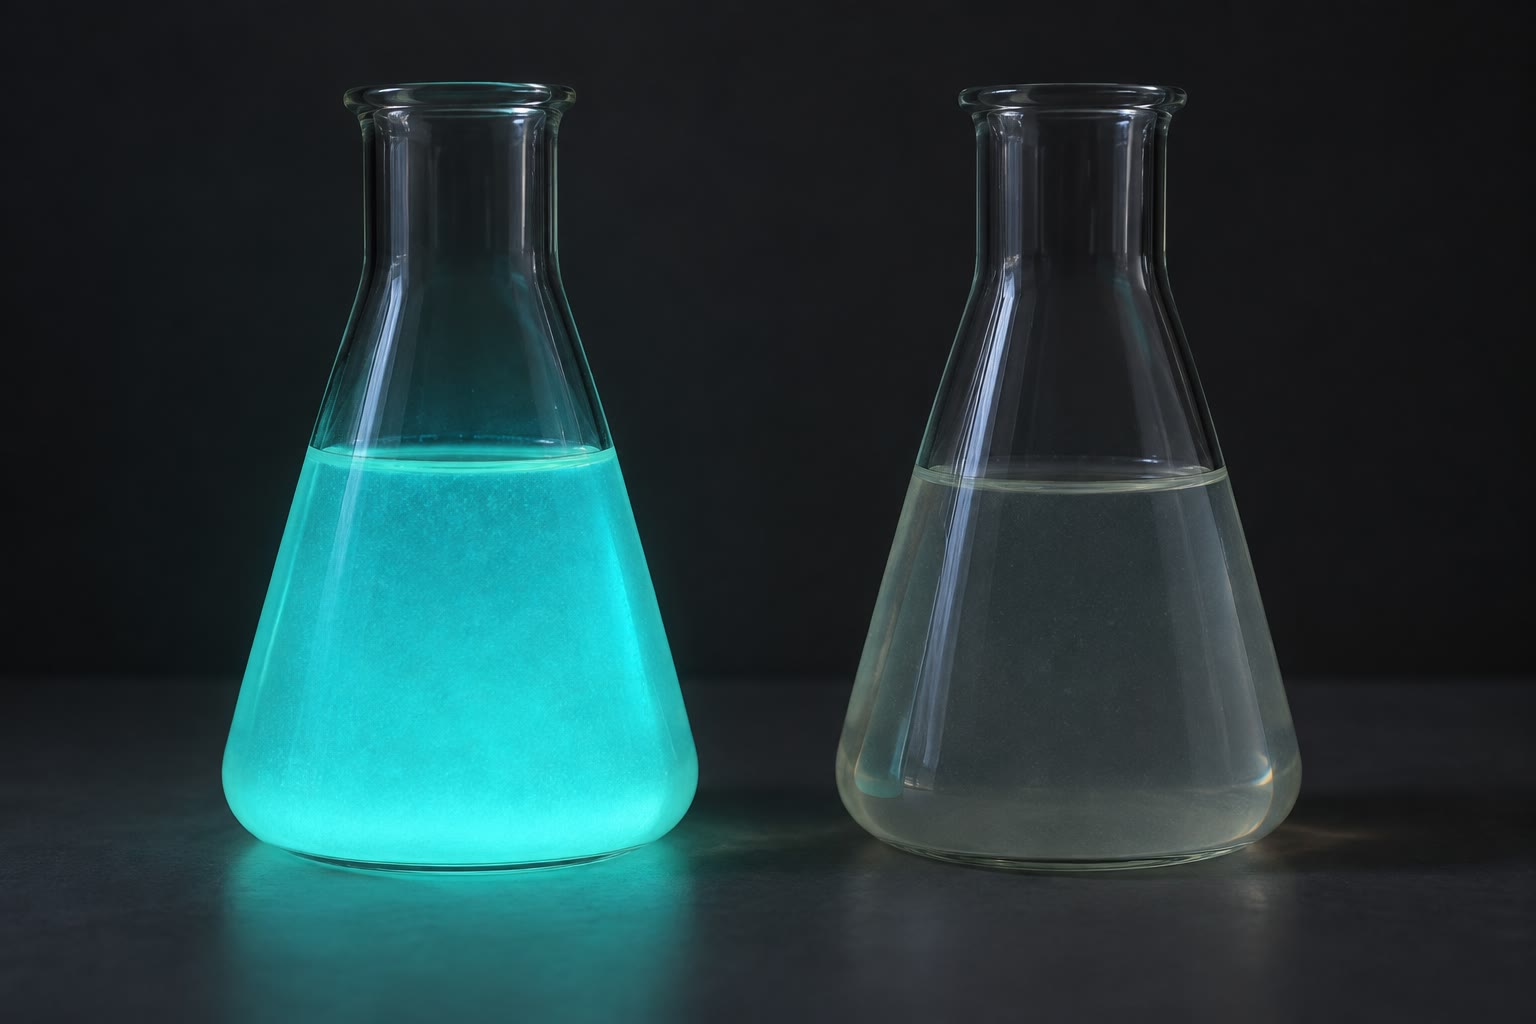
\includegraphics[width=0.46\linewidth]{images/book5/ai/b5-12-quorum-glow.jpg}\hspace{0.04\linewidth}
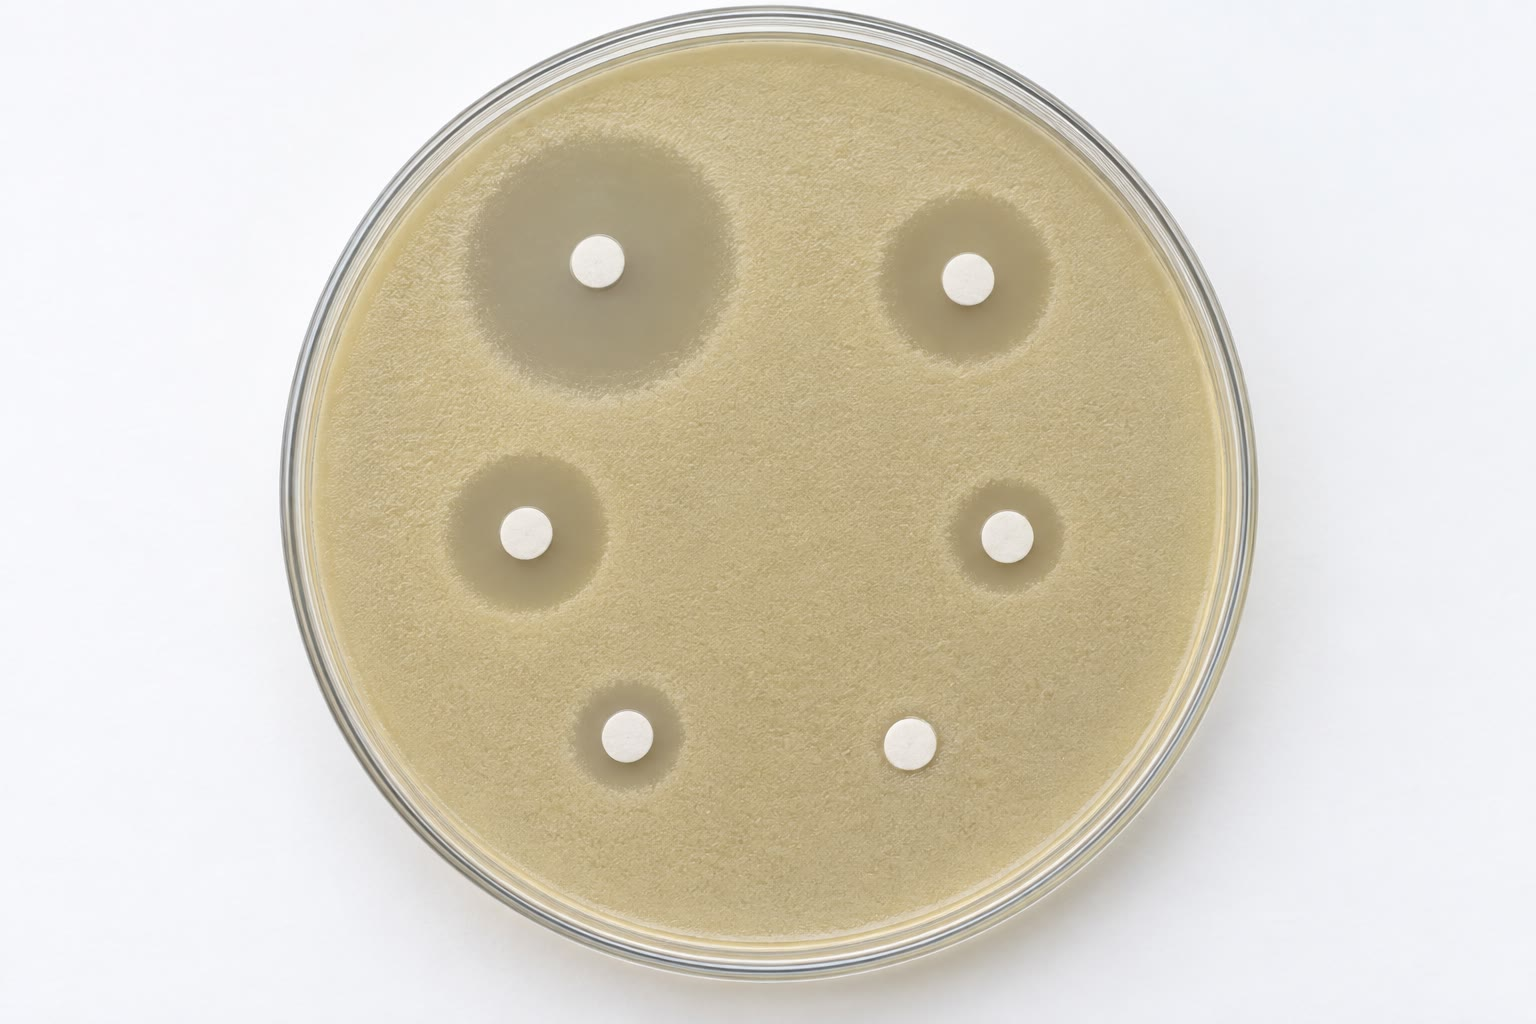
\includegraphics[width=0.46\linewidth]{images/book5/ai/b5-12-antibiotic-disks.jpg}

{\small À gauche~: une culture dense de \emph{Vibrio fischeri} qui
brille, à côté d'une culture diluée qui reste sombre --- les mêmes
cellules, au-dessus et au-dessous de leur quorum. À droite~: un test de
\omterm{met:b3:bacteriology:mic}{diffusion en disque}~; le diamètre de chaque zone claire mesure la
sensibilité de la bactérie à l'\omterm{def:b3:bacteriology:antibiotics}{antibiotique} du disque, et le disque sans
zone marque une résistance.}
\end{omfigure}

\section{Le trafic des gènes}

\begin{definition}[Transfert horizontal de gènes]\label{def:b3:bacteriology:hgt}
\index{transformation}\index{transduction}\index{conjugaison}\index{plasmide!de résistance}\index{élément génétique mobile}\index{pangénome}
Les bactéries se reproduisent clonalement mais échangent des gènes par
trois routes. La \emph{transformation}~: la capture d'ADN nu du milieu
par une cellule compétente --- la route par laquelle les pneumocoques
de Griffith ont acquis leur capsule et par laquelle Avery a montré que
le principe transformant était de l'ADN (1944). La
\emph{transduction}~: un phage qui emballe un morceau d'ADN de son hôte
et l'injecte dans le suivant (\cref{ch:b3:virology}). La
\emph{conjugaison}~: le transfert d'un \omterm{def:b3:genetic-engineering:tools}{plasmide} par un pilus et un pont
de conjugaison, d'un donneur qui le porte à un receveur, démontré par
Lederberg et Tatum (1946) avec des souches auxotrophes d'\emph{E.~coli}
qui ne donnaient de recombinants prototrophes qu'une fois mélangées.
Les \omterm{def:b3:genetic-engineering:tools}{plasmides} conjugatifs portent leurs propres gènes de transfert~;
beaucoup portent aussi des gènes de résistance, souvent groupés en
\emph{intégrons} et encadrés de transposons, de sorte qu'un seul
accouplement peut transférer la résistance à cinq \omterm{def:b3:bacteriology:antibiotics}{antibiotiques} à la
fois, par-delà les espèces. Il en résulte qu'une espèce bactérienne a
un génome cœur partagé par toutes ses souches et un génome accessoire
qui varie --- un \emph{pangénome}~: deux souches d'\emph{E.~coli}
peuvent différer par un cinquième de leurs gènes, et les souches
pathogènes diffèrent des souches inoffensives surtout par des îlots
acquis de gènes de virulence. Les gènes du chapitre des mutations du
volume de deuxième année naissent par mutation~; ceux de ce
chapitre-ci, pour la plupart, arrivent.
\end{definition}

\begin{omfigure}
\begin{tikzpicture}[every node/.style={font=\scriptsize}, >=stealth]
  % transformation
  \begin{scope}
    \draw[thick, fill=omDef!15] (0,0) ellipse (1.0 and 0.55);
    \draw[omThm, very thick] (-1.9,0.6) .. controls (-1.5,0.8) .. (-1.2,0.5); \draw[->, omThm, thick] (-1.2,0.5) -- (-0.7,0.25);
    \node[below, align=center] at (0,-0.7) {transformation~:\\de l'ADN nu capté\\par une cellule compétente};
  \end{scope}
  % transduction
  \begin{scope}[xshift=4.6cm]
    \draw[thick, fill=omDef!15] (0,0) ellipse (1.0 and 0.55);
    \draw[thick, fill=omProp!40] (-1.3,1.0) -- (-1.0,1.3) -- (-0.7,1.0) -- (-1.0,0.7) -- cycle; \draw[thick] (-1.0,0.7) -- (-0.9,0.35);
    \draw[omThm, very thick] (-1.1,1.15) -- (-0.9,0.85);
    \node[below, align=center] at (0,-0.7) {transduction~:\\un phage porte un morceau\\d'ADN de son hôte précédent};
  \end{scope}
  % conjugation
  \begin{scope}[xshift=9.6cm]
    \draw[thick, fill=omDef!15] (-1.3,0) ellipse (0.9 and 0.5); \draw[thick, fill=omDef!15] (1.3,0) ellipse (0.9 and 0.5);
    \draw[very thick, omMeth!70!black] (-0.4,0) -- (0.4,0);
    \draw[omThm, very thick] (-1.5,0) circle (0.25); \draw[->, omThm, thick] (-1.25,0) -- (1.0,0);
    \node[below, align=center] at (0,-0.7) {conjugaison~:\\un plasmide franchit\\un pont de conjugaison};
  \end{scope}
\end{tikzpicture}

{\small Les trois routes du transfert horizontal. Des gènes de
résistance, de virulence et de métabolisme passent de cellule à cellule
--- et d'espèce à espèce --- plus vite que la mutation ne saurait les
fabriquer.}
\end{omfigure}

\begin{proof}[Faits expérimentaux]
Robert Koch (1876--1884) a établi qu'une bactérie précise cause une
maladie précise~: il a isolé \emph{Bacillus anthracis} chez des animaux
malades, l'a cultivé en culture pure sur milieu solide (la boîte de
gélose et la colonie isolée sont des inventions de son laboratoire), a
montré que la culture reproduisait le charbon chez des animaux sains et
pouvait en être réisolée --- les postulats qui définissent encore un
pathogène --- puis est passé au bacille de la tuberculose et au vibrion
du choléra. Alexander Fleming (1928) a remarqué qu'une moisissure
contaminant une boîte de staphylocoques y avait dégagé une zone autour
d'elle~; la substance, la pénicilline, a été purifiée et s'est montrée
capable de guérir des infections chez Florey et Chain (1940--1941), et
en une décennie des staphylocoques résistants porteurs d'une enzyme qui
détruit la pénicilline étaient courants dans les hôpitaux --- un
avertissement que Fleming lui-même avait donné dans sa conférence
Nobel.
\end{proof}

\begin{omfigure}
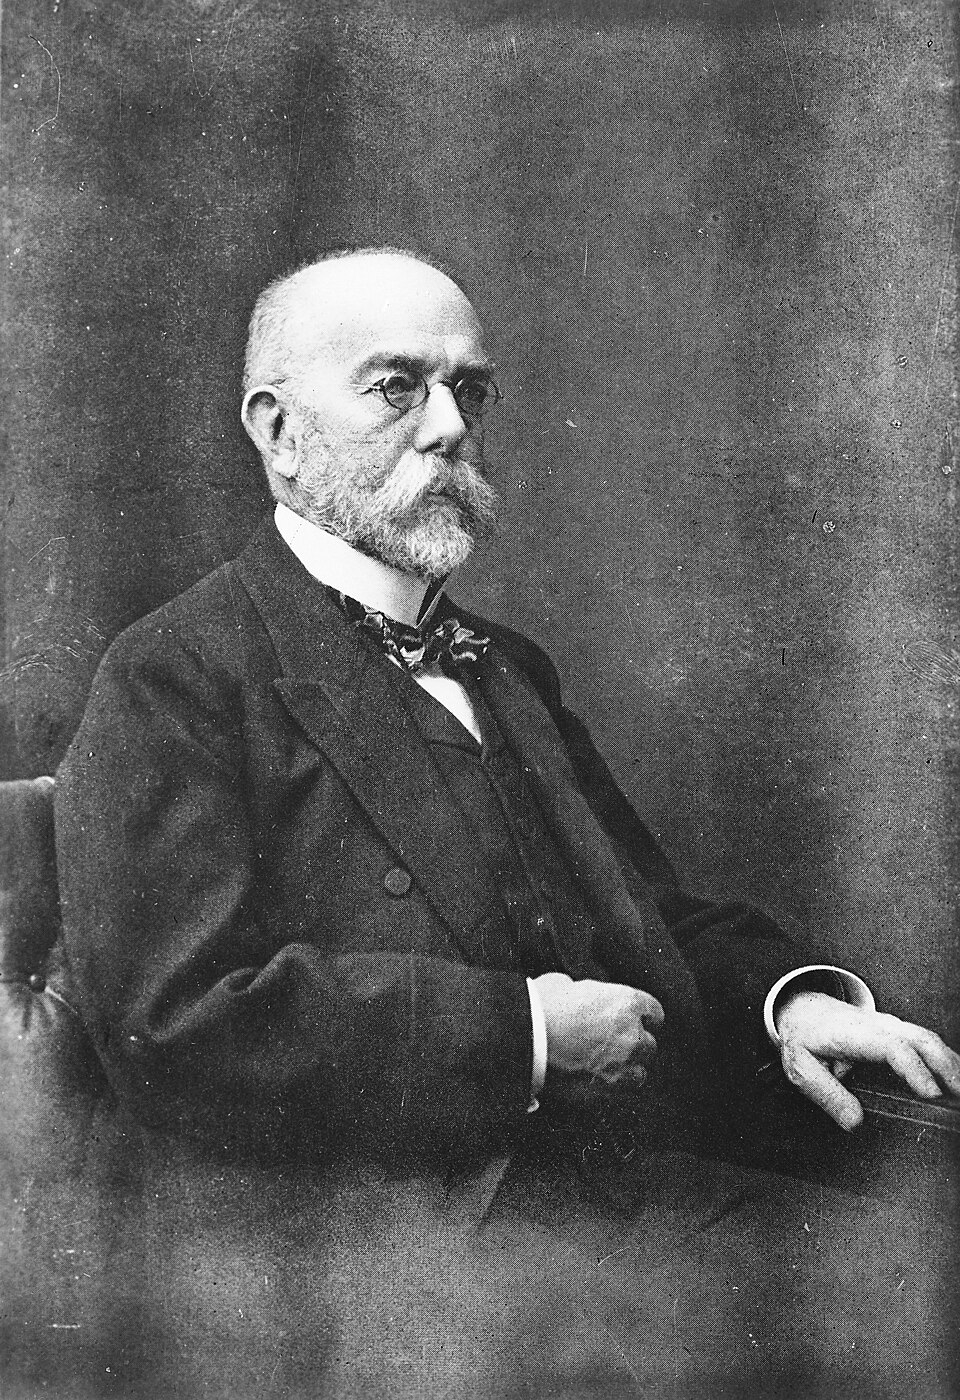
\includegraphics[width=0.30\linewidth]{images/book5/koch.jpg}\hspace{0.04\linewidth}
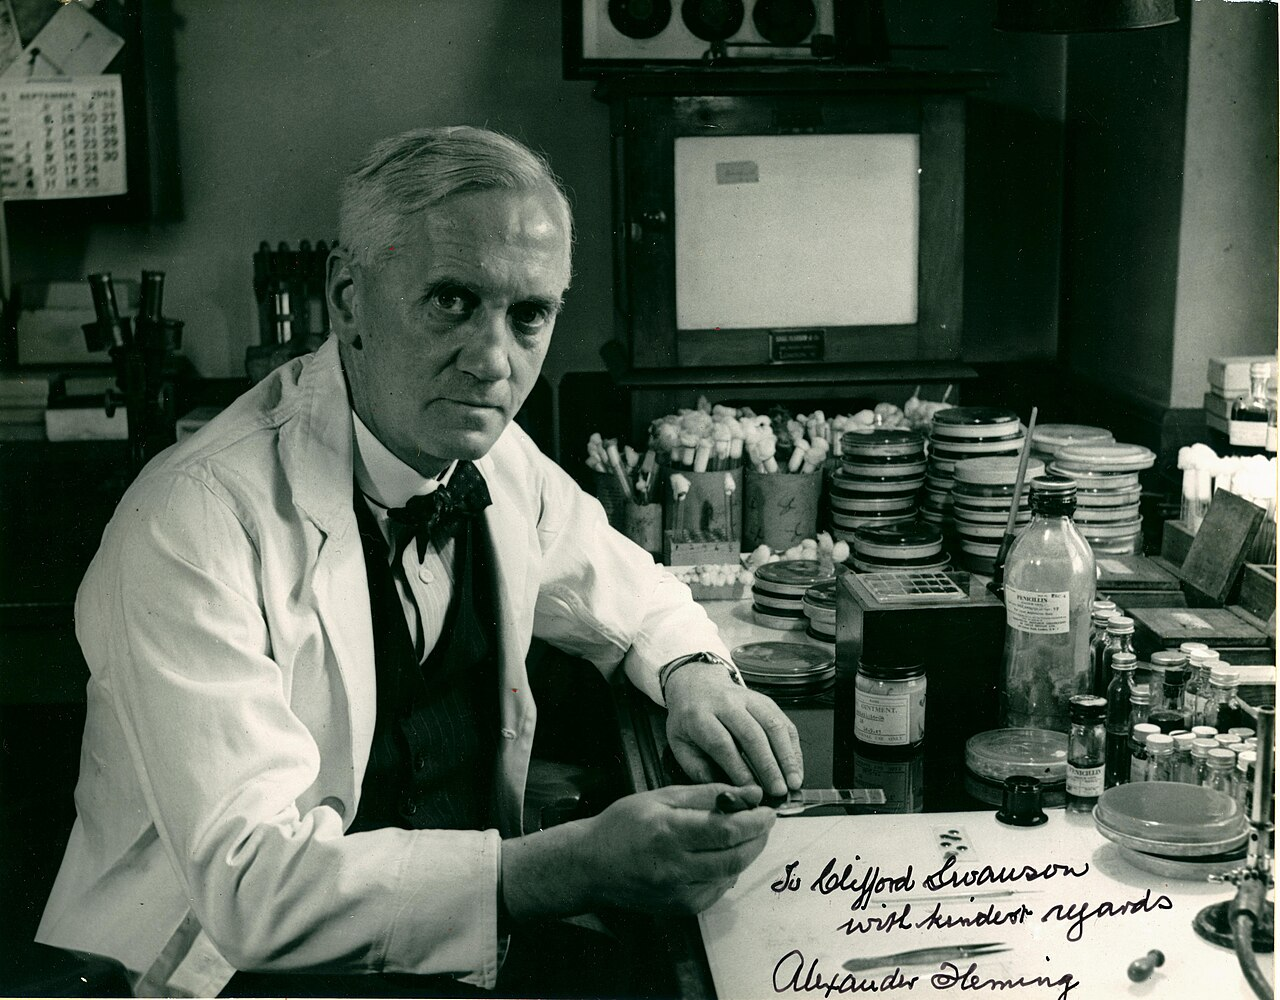
\includegraphics[width=0.56\linewidth]{images/book5/fleming.jpg}

{\small Robert Koch, qui a prouvé que des bactéries précises causent des
maladies précises et a inventé les méthodes pour les cultiver (Wellcome
Collection, CC~BY~4.0). À droite~: Alexander Fleming dans son
laboratoire, avec des boîtes de la moisissure dont le produit est
devenu la pénicilline (archives de l'U.S. Navy, domaine public).}
\end{omfigure}

\section{Antibiotiques et résistances}

\begin{definition}[Les antibiotiques]\label{def:b3:bacteriology:antibiotics}
\index{antibiotique}\index{bêta-lactamine}\index{toxicité sélective}\index{concentration minimale inhibitrice}
Un \emph{antibiotique} est une molécule qui tue les bactéries ou arrête
leur croissance à des concentrations inoffensives pour l'hôte, en
agissant sur une cible que l'hôte n'a pas ou qu'il a sous une autre
forme --- la \emph{toxicité sélective}. Les cibles sont peu
nombreuses. La paroi~: les \emph{$\beta$-lactamines} (pénicillines,
céphalosporines, carbapénèmes) imitent le D-Ala-D-Ala terminal du
peptide du \omterm{def:b3:bacteriology:envelope}{peptidoglycane} et acylent les enzymes qui le réticulent, de
sorte que la paroi en croissance est faible et que la cellule éclate
sous sa propre turgescence~; la vancomycine se fixe sur le D-Ala-D-Ala
lui-même. Le ribosome, dont la forme bactérienne diffère de
l'eucaryote~: les aminosides (la petite sous-unité, d'où des erreurs de
lecture), les tétracyclines (qui bloquent l'entrée des ARNt), les
macrolides et le chloramphénicol (le tunnel de sortie et la
peptidyl-transférase de la grande sous-unité). L'ADN gyrase et la
topo-isomérase~IV~: les quinolones. L'ARN polymérase~: la rifampicine.
La synthèse des folates, que les animaux ne font pas~: les sulfamides
et le triméthoprime. La membrane~: les polymyxines, en dernier
recours. La \emph{concentration minimale inhibitrice} (CMI) est la plus
faible concentration d'un médicament qui empêche la croissance visible
d'une souche~; une souche est dite résistante quand sa CMI dépasse la
concentration que le médicament atteint chez le patient.
\end{definition}

\begin{method}[Mesurer la sensibilité]\label{met:b3:bacteriology:mic}
\index{diffusion en disque}\index{dilution en bouillon}
Deux tests. La \emph{\omterm{met:b3:bacteriology:mic}{dilution en bouillon}}~: ensemencer un nombre fixe
de cellules (environ $5\times 10^{5}$ par millilitre) dans une rangée
de tubes ou de puits contenant l'\omterm{def:b3:bacteriology:antibiotics}{antibiotique} par paliers de facteur
deux, incuber une nuit, et lire le premier puits clair~: cette
concentration est la CMI. La \emph{\omterm{met:b3:bacteriology:mic}{diffusion en disque}}~: étaler la
souche sur une boîte de gélose, poser des disques de papier chargés de
quantités connues de plusieurs \omterm{def:b3:bacteriology:antibiotics}{antibiotiques}, incuber~; le médicament
diffuse vers l'extérieur, sa concentration décroissant avec la
distance, et la croissance est inhibée jusqu'au rayon où la
concentration égale la CMI, de sorte que le diamètre de la zone claire
--- lu sur des tables étalonnées --- donne la sensibilité à chaque
disque sur une seule boîte. Les deux tests prennent un jour~; séquencer
le génome à la recherche des gènes et des mutations de résistance
connus prend le même jour et commence à les remplacer.
\end{method}

\begin{definition}[La résistance]\label{def:b3:bacteriology:resistance}
\index{résistance aux antibiotiques}\index{bêta-lactamase}\index{pompe d'efflux}\index{SARM}
Une bactérie résiste à un \omterm{def:b3:bacteriology:antibiotics}{antibiotique} par l'un de cinq moyens. Elle
détruit le médicament~: les \emph{$\beta$-lactamases} hydrolysent le
cycle $\beta$-lactame, et les variantes à spectre étendu et les
carbapénémases détruisent aujourd'hui les plus récentes. Elle modifie
la cible~: une mutation de la protéine ribosomique ou de la gyrase que
le médicament fixe, ou bien, chez le SARM (\emph{Staphylococcus aureus}
résistant à la méticilline), un gène acquis codant une enzyme de
réticulation que les $\beta$-lactamines ne fixent pas~; la résistance à
la vancomycine remplace le D-Ala terminal par un D-lactate, que le
médicament ne reconnaît pas. Elle chasse le médicament par des
\emph{pompes d'efflux}, souvent de spécificité large. Elle empêche le
médicament d'entrer, en perdant une porine. Ou elle contourne l'étape
bloquée par une autre enzyme. Les mutations de cible apparaissent par
hasard chez le patient à des taux de $10^{-8}$ à $10^{-6}$ par
division et sont sélectionnées pendant le traitement~; les enzymes et
les pompes sont surtout acquises sur des \omterm{def:b3:genetic-engineering:tools}{plasmides} venus de l'immense
réservoir des bactéries du sol et de l'intestin, où elles ont évolué
depuis des âges contre les \omterm{def:b3:bacteriology:antibiotics}{antibiotiques} que fabriquent les
champignons et d'autres bactéries. Les persistantes --- cellules
dormantes qui survivent à un médicament sans être génétiquement
résistantes --- expliquent les rechutes après un traitement qui aurait
dû réussir.
\end{definition}

\begin{proposition}[Pourquoi la résistance est inévitable et l'association la réponse]\label{prop:b3:bacteriology:selection}
\index{résistance!sélection}\index{polythérapie!antibiotiques}
Une infection de $10^{9}$ cellules traitée par un médicament contre
lequel les mutations de résistance apparaissent à $10^{-8}$ par
division contient déjà une dizaine de cellules résistantes~; le
médicament tue le reste et les dix prennent la place --- exactement
l'arithmétique du \cref{ch:b3:cancer-biology}, puisqu'une population
bactérienne et une \omterm{def:b3:cancer-biology:hallmarks}{tumeur} sont l'une comme l'autre des clones qui
évoluent sous sélection. Deux médicaments à cibles indépendantes
affrontent une cellule doublement résistante à $10^{-16}$ par division,
qu'un milliard de cellules ne contient pas. C'est pourquoi la
tuberculose, dont les lésions abritent $10^{8}$--$10^{9}$ bacilles, est
traitée par trois ou quatre médicaments à la fois depuis les années
1950 et pourquoi sa monothérapie a produit des résistances en quelques
mois~; c'est aussi pourquoi chaque emploi d'un \omterm{def:b3:bacteriology:antibiotics}{antibiotique}, chez un
patient ou dans un élevage, sélectionne de la résistance quelque part,
et pourquoi le rythme des \omterm{def:b3:bacteriology:antibiotics}{antibiotiques} nouveaux --- aucune classe
nouvelle contre les \omterm{def:b3:bacteriology:envelope}{Gram négatifs} depuis les années 1960 --- est la
mesure à laquelle on compte les pertes. Les remèdes sont ceux de tout
affrontement évolutif~: en employer moins, associer, terminer la cure
pour que des cellules partiellement résistantes ne survivent pas à se
reproduire, et trouver de nouvelles cibles.
\end{proposition}

\begin{example}[La fenêtre de sélection des mutants]\label{ex:b3:bacteriology:window}
Une souche a une CMI de \qty{1}{mg/L}~; ses mutants résistants de
premier rang, présents à raison d'un sur $10^{7}$, ont une CMI de
\qty{8}{mg/L}. Une dose qui maintient le médicament à \qty{4}{mg/L} tue
le type sauvage et laisse les mutants croître sans concurrence~:
l'intervalle de concentration compris entre la CMI du type sauvage et
celle des mutants est la \emph{fenêtre de sélection des mutants}, et un
traitement qui s'y installe fabrique de la résistance. Une dose
au-dessus de \qty{8}{mg/L} tue les deux~; une dose trop faible, ou une
cure arrêtée quand le patient se sent mieux et que la concentration
redescend à travers la fenêtre, voilà comment se fabrique une
population résistante. La même logique fixe les protocoles du
traitement de la tuberculose~: six mois, quatre médicaments, à des
doses supérieures à la CMI de tout mutant en un pas.
\end{example}

\begin{omfigure}
\begin{tikzpicture}
\begin{axis}[
  width=0.7\linewidth, height=5.6cm,
  axis x line=bottom, axis y line=left,
  xmin=0, xmax=24, ymin=0.25, ymax=32, ymode=log,
  xlabel={heures après une dose}, ylabel={médicament plasmatique (mg/L)},
  xlabel style={font=\small, at={(axis description cs:0.5,-0.12)}, anchor=north}, ylabel style={font=\small},
  tick label style={font=\small}, xtick={0,6,12,18,24}, ytick={0.5,1,2,4,8,16}, yticklabels={0.5,1,2,4,8,16},
  clip=false,
]
\fill[omThm!15] (axis cs:0,1) rectangle (axis cs:24,8);
\addplot[very thick, omDef, domain=0:24, samples=60] {16*exp(-0.15*x)};
\addplot[dashed, gray, domain=0:24, samples=2] {1}; \addplot[dashed, gray, domain=0:24, samples=2] {8};
\node[font=\scriptsize, gray, anchor=south west] at (axis cs:0.3,1.05) {CMI du type sauvage};
\node[font=\scriptsize, gray, anchor=south east] at (axis cs:23.7,8.4) {CMI du mutant de premier rang};
\node[font=\scriptsize, omThm!70!black, anchor=west] at (axis cs:13,3.5) {fenêtre de sélection des mutants};
\node[font=\scriptsize, omDef, anchor=south west] at (axis cs:2,13) {concentration plasmatique après une dose};
\end{axis}
\end{tikzpicture}

{\small La fenêtre de sélection des mutants. Une concentration
supérieure à la CMI des mutants tue tout~; entre les deux CMI (zone
grisée) elle tue le type sauvage et sélectionne les mutants. Une dose
dont la concentration traverse la fenêtre pendant des heures, ou une
cure arrêtée trop tôt, fabrique de la résistance.}
\end{omfigure}

\begin{remark}[La plupart des bactéries ne sont pas des pathogènes]\label{rem:b3:bacteriology:most}
Les bactéries de la clinique de ce chapitre sont une infime minorité.
Sur le million d'espèces estimées, quelques centaines causent des
maladies humaines~; les autres font tourner les cycles de l'azote, du
soufre et du carbone (le volume de deuxième année), fixent l'azote de
chaque légumineuse, digèrent la cellulose de chaque ruminant, et
composent les microbiotes du \cref{ch:b3:microbiomes}, dont la perte
sous \omterm{def:b3:bacteriology:antibiotics}{antibiotique} est un coût de chaque cure. Les \omterm{def:b3:bacteriology:antibiotics}{antibiotiques}
eux-mêmes sont leurs molécules --- armes et signaux évolués parmi les
bactéries et les champignons du sol bien avant qu'il y ait des hôpitaux
--- et la plupart des gènes de résistance aussi.
\end{remark}

\section{Exercices}

\begin{exercise}[$\star$]\label{exo:b3:bacteriology:1}
Décrire les enveloppes à \omterm{def:b3:bacteriology:envelope}{Gram positif} et à \omterm{def:b3:bacteriology:envelope}{Gram négatif} et expliquer
pourquoi la \omterm{met:b3:bacteriology:gram}{coloration de Gram} les distingue.
\end{exercise}

\begin{exercise}[$\star$]\label{exo:b3:bacteriology:2}
Une culture de $10^{3}$ cellules par millilitre atteint $10^{9}$ en
\qty{8}{h} de croissance exponentielle. Trouver le nombre de
générations, le temps de génération et $\mu$.
\end{exercise}

\begin{exercise}[$\star$]\label{exo:b3:bacteriology:3}
Nommer les trois routes du transfert horizontal de gènes et donner
l'expérience classique qui a démontré chacune.
\end{exercise}

\begin{exercise}[$\star$]\label{exo:b3:bacteriology:4}
Donner la cible de la pénicilline, de la streptomycine, de la
ciprofloxacine et de la rifampicine, et dire pourquoi chacune est
sélectivement toxique.
\end{exercise}

\begin{exercise}[$\star\star$]\label{exo:b3:bacteriology:5}
Un chémostat a $\mu_{\max} = \qty{0.8}{h^{-1}}$, $K_{S} =
\qty{0.02}{g/L}$, $S_{0} = \qty{2}{g/L}$, $Y = 0.4$. Calculer $S^{*}$ et
$X^{*}$ en $D = 0.2$, $0.6$ et $0.79$ h$^{-1}$, ainsi que le \omterm{thm:b3:bacteriology:monod}{taux de
dilution} auquel commence le lessivage.
\end{exercise}

\begin{exercise}[$\star\star$]\label{exo:b3:bacteriology:6}
À l'aide de la \cref{prop:b3:bacteriology:threshold}, comparer la
densité seuil de la \omterm{def:b3:bacteriology:quorum}{détection du quorum} dans l'organe lumineux d'un
calmar ($k =
\qty{0.01}{h^{-1}}$) et dans une eau de mer courante
($k = \qty{10}{h^{-1}}$), avec $p = 100$ molécules par cellule et par
heure et $A_{\text{seuil}} =
\qty{10}{nmol/L}$ ($6\times 10^{12}$ molécules par litre).
\end{exercise}

\begin{exercise}[$\star\star$]\label{exo:b3:bacteriology:7}
Une boîte de \omterm{met:b3:bacteriology:mic}{diffusion en disque} montre des zones de $25$, $12$ et
\qty{0}{mm} pour trois médicaments. Interpréter chacune, et expliquer
pourquoi un diamètre de zone peut être converti en CMI.
\end{exercise}

\begin{exercise}[$\star\star$]\label{exo:b3:bacteriology:8}
Expliquer comment un seul événement de \omterm{def:b3:bacteriology:hgt}{conjugaison} peut rendre une
\emph{Klebsiella} sensible résistante à cinq \omterm{def:b3:bacteriology:antibiotics}{antibiotiques}, et pourquoi
les gènes de résistance se trouvent si souvent groupés sur des
\omterm{def:b3:genetic-engineering:tools}{plasmides}.
\end{exercise}

\begin{exercise}[$\star\star$]\label{exo:b3:bacteriology:9}
Un patient porte $10^{9}$ bactéries et prend un médicament contre
lequel la résistance apparaît à $10^{-7}$ par division. Calculer le
nombre attendu de cellules résistantes au départ~; puis avec deux
médicaments indépendants. Pourquoi les persistantes sont-elles un
problème différent~?
\end{exercise}

\begin{exercise}[$\star\star\star$]\label{exo:b3:bacteriology:10}
Montrer que l'état stationnaire du chémostat est stable~: perturber $X$
légèrement au-dessus de $X^{*}$ et suivre les signes de
$\mathrm{d}S/\mathrm{d}t$ et de $\mathrm{d}X/\mathrm{d}t$. Expliquer
ensuite pourquoi deux espèces qui se disputent un même nutriment dans
un chémostat ne peuvent pas coexister à l'état stationnaire, et
laquelle l'emporte à un $D$ donné.
\end{exercise}

\begin{exercise}[$\star\star\star$]\label{exo:b3:bacteriology:11}
L'\omterm{def:b3:bacteriology:quorum}{auto-inducteur} induit sa propre synthase. Modifier le modèle de la
\cref{prop:b3:bacteriology:threshold} de sorte que $p$ saute de $p_{0}$
à $p_{1} \gg p_{0}$ quand $A > A_{\text{seuil}}$, et montrer que le
système peut avoir deux états stables sur une plage de densités
(hystérésis)~: une population qui s'est allumée reste allumée à une
densité où une population naïve serait éteinte. Quelle en est l'utilité
biologique~?
\end{exercise}

\begin{exercise}[$\star\star\star$]\label{exo:b3:bacteriology:12}
Expliquer la fenêtre de sélection des mutants et s'en servir pour
plaider pour ou contre chacun de ces choix~: (a) de fortes doses en
cures courtes~; (b) de faibles doses en cures longues~; (c) arrêter
quand les symptômes cèdent~; (d) l'association de médicaments.
\end{exercise}

\section{Problème~: un chémostat et une clinique}

\begin{problem}[{Problème du week-end --- une culture menée en flacon
puis maintenue dans un chémostat, une bactérie lumineuse comptée
jusqu'à son quorum, et une infection traitée contre l'arithmétique de
la résistance, pour finir sur les cellules du chémostat, la densité à
laquelle la lumière s'allume et les chances qu'une cure à deux
médicaments rencontre une cellule résistante}]
\label{pb:b3:bacteriology:1}
Données~: \emph{E.~coli} à \qty{37}{\celsius}, $T = \qty{20}{min}$~; une
cellule pèse \qty{1}{pg}. Chémostat~: $V = \qty{1}{L}$,
$F = \qty{0.5}{L/h}$, $\mu_{\max} = \qty{1.0}{h^{-1}}$,
$K_{S} = \qty{0.01}{g/L}$, $S_{0} =
\qty{2}{g/L}$ de glucose, $Y = 0.5$. \emph{Vibrio}~: $p = 500$
molécules d'\omterm{def:b3:bacteriology:quorum}{auto-inducteur} par cellule et par heure,
$A_{\text{seuil}} = 6\times 10^{12}$ molécules par litre
(\qty{10}{nmol/L}), $k = \qty{0.05}{h^{-1}}$ dans l'organe lumineux.
Infection~: $10^{9}$ cellules~; résistance au médicament A à $10^{-8}$
par division, au médicament B à $10^{-7}$~; CMI du type sauvage pour A
\qty{1}{mg/L}, mutant de premier rang \qty{8}{mg/L}~; une dose donne
\qty{16}{mg/L} qui décroît avec une demi-vie de \qty{4}{h}.

\medskip
\noindent\textbf{Partie I --- Le flacon.}
\begin{enumerate}
  \item Une cellule dans \qty{100}{mL} de bouillon. Combien de cellules
        après \qty{6}{h} de croissance exponentielle, et quelle densité
        par mL~?
  \item Le bouillon ne supporte au plus que $2\times 10^{9}$ cellules
        par mL. Quand la croissance s'arrête-t-elle, et quelle est la
        masse de cellules de la culture~?
  \item Combien de temps faudrait-il à la descendance d'une cellule
        pour atteindre la masse de la Terre ($6\times 10^{27}$ g)~?
        Commenter.
  \item La \omterm{def:b3:bacteriology:phases}{phase de latence} dure \qty{1}{h} quand on ensemence du
        milieu neuf avec des cellules de \omterm{def:b3:bacteriology:phases}{phase stationnaire}, et presque
        rien avec des cellules exponentielles. Expliquer.
  \item Calculer $\mu$ à partir de $T$. Si l'on passe à un sucre sur
        lequel $T = \qty{60}{min}$, que vaut $\mu$, et de quel facteur
        le nombre de cellules après \qty{6}{h} diminue-t-il~?
  \item Un échantillon de la culture stationnaire est étalé sur une
        boîte et donne $200$ colonies à partir de \qty{0.1}{mL} d'une
        dilution au $10^{-6}$. Quel est le compte de cellules viables,
        et pourquoi peut-il différer d'un comptage au microscope~?
\end{enumerate}

\medskip
\noindent\textbf{Partie II --- Le chémostat.}
\begin{enumerate}[resume]
  \item Calculer le \omterm{thm:b3:bacteriology:monod}{taux de dilution} $D$ et le temps de génération que
        la culture est forcée d'adopter.
  \item Calculer $S^{*}$ et $X^{*}$ (en g/L et en cellules par mL).
  \item Combien de cellules quittent la cuve par heure~? Combien de
        générations la culture traverse-t-elle en un mois~?
  \item On monte la pompe à $F = \qty{0.95}{L/h}$. Nouveaux $S^{*}$ et
        $X^{*}$~? Que se passe-t-il à $F = \qty{1.1}{L/h}$~?
  \item Un mutant apparaît avec $\mu_{\max} = \qty{1.2}{h^{-1}}$ et le
        même $K_{S}$. À $D = 0.5$, de quel $S^{*}$ a-t-il besoin, et
        qu'advient-il de la souche d'origine~? (Utiliser
        l'\cref{exo:b3:bacteriology:10}.)
  \item Un mois de fonctionnement fait $700$ générations. Si une
        mutation avantageuse apparaît à $10^{-9}$ par division et que
        la cuve contient $10^{12}$ cellules, combien de mutations
        avantageuses apparaissent par génération~? Que dit cela de
        l'évolution dans un chémostat~?
\end{enumerate}

\medskip
\noindent\textbf{Partie III --- Le quorum.}
\begin{enumerate}[resume]
  \item Calculer la densité cellulaire seuil pour la lumière dans
        l'organe lumineux, en cellules par mL.
  \item L'organe lumineux contient \qty{1}{\micro L} de bactéries à
        $10^{10}$ par mL. De quel facteur l'\omterm{def:b3:bacteriology:quorum}{auto-inducteur} dépasse-t-il
        le seuil~?
  \item En mer, le signal est emporté avec $k = \qty{20}{h^{-1}}$.
        Densité seuil~? Comparer aux $10^{2}$ cellules par mL du large.
  \item Après que le calmar a expulsé \qty{90}{\%} des bactéries à
        l'aube, combien de temps faut-il aux $10^{9}$ par mL restantes,
        qui se divisent toutes les \qty{2}{h}, pour rétablir $10^{10}$
        par mL~? La lumière s'éteint-elle entre-temps~?
  \item Chaque cellule qui brille dépense environ \qty{20}{\%} de son
        énergie en lumière. Pourquoi une cellule sombre est-elle
        favorisée en mer, et pourquoi pas dans l'organe~?
  \item Un pathogène emploie le même système pour retarder ses toxines
        jusqu'à ce qu'il soit nombreux. Proposer une stratégie
        médicamenteuse qui l'exploite et dire pourquoi elle
        sélectionnerait la résistance plus lentement qu'un
        \omterm{def:b3:bacteriology:antibiotics}{antibiotique}.
\end{enumerate}

\medskip
\noindent\textbf{Partie IV --- La clinique.}
\begin{enumerate}[resume]
  \item Nombre attendu de cellules résistantes à A au début du
        traitement~; à B~; aux deux.
  \item Probabilité qu'aucune cellule résistante à A n'existe~; aux
        deux.
  \item Après la dose, quand la concentration tombe-t-elle à
        \qty{8}{mg/L}, puis à \qty{1}{mg/L}~? Combien de temps par dose
        passe-t-elle dans la fenêtre de sélection des mutants~?
  \item Si le médicament est donné toutes les \qty{12}{h}, quelle
        fraction du temps la concentration est-elle dans la fenêtre, et
        que cela prédit-il au cours d'une cure de dix jours avec A
        seul~?
  \item Proposer un changement de posologie qui maintienne la
        concentration au-dessus de \qty{8}{mg/L} en permanence
        (calculer l'intervalle ou la dose nécessaire), et en dire le
        coût.
  \item Une cellule sur $10^{4}$ est une persistante, dormante et
        insensible à toute concentration de l'un ou l'autre médicament.
        Combien en survivent à la cure, que se passe-t-il au retrait du
        médicament, et qu'est-ce que cela implique pour la durée du
        traitement~?
  \item Résumer~: les cellules par mL du chémostat (question~8), la
        densité seuil de la lumière (question~13) et la probabilité que
        la cure à deux médicaments ne rencontre aucune cellule
        résistante (question~20).
\end{enumerate}
\end{problem}
